%% Lecture 13 -- Bernoulli's Equation and Applications

\documentclass[../main.tex]{subfiles}
\begin{document}

\section{Lecture 13 -- Bernoulli's Equation and Applications}\label{sec:lec13}
\begin{center}
  \textbf{Date:} May 20, 2026
\end{center}

\subsection*{Overview}
This lecture has two goals. First, we re-derive Bernoulli's equation carefully, including the gravitational-potential term that was omitted in the previous session. Second, we apply it to three canonical problems: a draining tank (Torricelli's theorem), the Venturi effect, and the lift on an airfoil. The lecture closes with a preview of the next topic: systematic derivation of conservation laws from an action principle, which requires switching from the Eulerian to the Lagrangian description of fluid motion.

% ──────────────────────────────────────────────────────────────────────────────
\subsection{Complete Derivation of Bernoulli's Equation}\label{sec:lec13:bernoulli}
% ──────────────────────────────────────────────────────────────────────────────

\subsubsection*{Physical Motivation}
Bernoulli's equation is the energy-conservation law of an ideal fluid along a streamline. Last lecture the derivation was done rapidly and the gravitational potential term was dropped. We now redo it from scratch. Euler's equation is the starting point; dotting it with the velocity vector converts a force law into an energy law, exactly as in particle mechanics.

\subsubsection{Setup: Steady Flow with a Conservative Body Force}
We assume
\begin{itemize}
  \item \emph{Steady flow}: all partial time derivatives vanish, $\partial_t(\cdot)=0$.
  \item \emph{Ideal (inviscid) fluid}: stress is purely isotropic, $\sigma_{ij}=-p\delta_{ij}$.
  \item \emph{Conservative body force}: the body-force acceleration is $\bvec{g}=-\grad\Phi$, where $\Phi(\bvec{x})$ is the external potential (e.g.\ $\Phi=gz$ for uniform gravity).
  \item \emph{Barotropic fluid}: pressure and density satisfy $p=p(\rho)$, so the specific enthalpy
    \[
      h_{\mathrm{th}}=\int\frac{dp}{\rho(p)}
    \]
    is well-defined, and $\grad h_{\mathrm{th}}=\frac{1}{\rho}\grad p$.
\end{itemize}

Euler's equation is
\begin{equation}
  \pdv{\vel}{t}+(\vel\cdot\grad)\vel = -\frac{1}{\rho}\grad p + \bvec{g}.
  \label{eq:lec13_euler}
\end{equation}
Under steady flow $\partial_t\vel=0$, and substituting the conservative body force,
\begin{equation}
  (\vel\cdot\grad)\vel = -\grad h_{\mathrm{th}} - \grad\Phi.
  \label{eq:lec13_euler_steady}
\end{equation}

\subsubsection{Dot with $\vel$}
Take the scalar product of \eqref{eq:lec13_euler_steady} with $\vel$:
\begin{align}
  \vel\cdot\bigl[(\vel\cdot\grad)\vel\bigr]
  &= -\vel\cdot\grad h_{\mathrm{th}} - \vel\cdot\grad\Phi.
  \label{eq:lec13_dot_1}
\end{align}
The left side simplifies because
\begin{equation}
  \vel\cdot\bigl[(\vel\cdot\grad)\vel\bigr]
  = (\vel\cdot\grad)\tfrac{1}{2}v^2.
  \label{eq:lec13_kinetic_identity}
\end{equation}
For steady flow, $\partial_t=0$, so the material derivative satisfies $\DDt(\cdot)=\vel\cdot\grad(\cdot)$. Thus the right side can also be written as material derivatives:
\begin{align}
  \vel\cdot\grad h_{\mathrm{th}} &= \DDt h_{\mathrm{th}},\\
  \vel\cdot\grad\Phi &= \DDt\Phi.
\end{align}
(These equalities rely on steady flow, i.e., $\partial_t h_{\mathrm{th}}=\partial_t\Phi=0$.)

Equation \eqref{eq:lec13_dot_1} therefore becomes
\begin{equation}
  \DDt\!\left(\frac{1}{2}v^2\right) = -\DDt h_{\mathrm{th}} - \DDt\Phi,
\end{equation}
which rearranges to
\begin{equation}
  \DDt\!\left(\frac{1}{2}v^2 + h_{\mathrm{th}} + \Phi\right) = 0.
  \label{eq:lec13_bernoulli_material}
\end{equation}
The material derivative is zero along the path of any fluid element, so the quantity in the parenthesis is constant along every streamline:

\thm[bernoulli]{Bernoulli's Equation (general barotropic form)}{%
  For steady, ideal, barotropic flow in a conservative external field $\Phi$,
  \begin{equation}
    \boxed{\frac{1}{2}v^2 + h_{\mathrm{th}} + \Phi = \mathrm{const\ along\ a\ streamline},}
    \label{eq:lec13_bernoulli_general}
  \end{equation}
  where $h_{\mathrm{th}}=\int dp/\rho$ is the specific enthalpy and $\Phi$ is the external potential.
}
\textit{Significance:} The three terms are kinetic energy per unit mass, pressure-work energy per unit mass, and gravitational potential energy per unit mass. Their sum is conserved along any streamline. The previously missing term is $\Phi$.

\subsubsection{Important Special Cases}

\paragraph{Incompressible fluid with uniform gravity.}
For $\rho=\rho_0=\mathrm{const}$, $h_{\mathrm{th}}=p/\rho_0$, and $\Phi=gz$:
\begin{equation}
  \boxed{\frac{1}{2}v^2 + \frac{p}{\rho_0} + gz = \mathrm{const\ along\ a\ streamline}.}
  \label{eq:lec13_bernoulli_incompressible}
\end{equation}
Multiplied by $\rho_0$,
\begin{equation}
  \boxed{\frac{1}{2}\rho_0 v^2 + p + \rho_0 gz = \mathrm{const.}}
  \label{eq:lec13_bernoulli_pressure_form}
\end{equation}

\paragraph{Static limit ($\vel=0$).}
The kinetic term vanishes and Bernoulli reduces to the hydrostatic equation:
\begin{equation}
  p + \rho_0 gz = \mathrm{const} \quad\Longrightarrow\quad \grad p = -\rho_0 g\,\uvec{z} = \rho_0\bvec{g}.
\end{equation}
\textit{Significance:} Bernoulli unifies hydrostatics and free-fall energy conservation into one equation.

\paragraph{Physical interpretation.}
Bernoulli = hydrostatics + free-fall in two limits:
\begin{center}
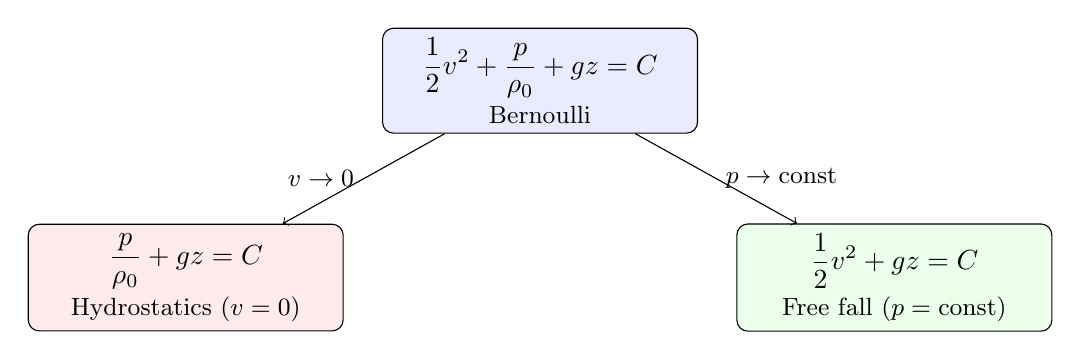
\begin{tikzpicture}
  \node[draw, rounded corners, fill=blue!8, minimum width=4cm, minimum height=1.1cm, align=center]
    (B) at (0,0) {$\displaystyle\frac{1}{2}v^2 + \frac{p}{\rho_0} + gz = C$\\[2pt] \small Bernoulli};
  \node[draw, rounded corners, fill=red!8, minimum width=4cm, minimum height=1.0cm, align=center]
    (H) at (-4.5,-2.5) {$\displaystyle\frac{p}{\rho_0} + gz = C$\\[2pt]\small Hydrostatics ($v=0$)};
  \node[draw, rounded corners, fill=green!8, minimum width=4cm, minimum height=1.0cm, align=center]
    (F) at (4.5,-2.5) {$\displaystyle\frac{1}{2}v^2 + gz = C$\\[2pt]\small Free fall ($p=\mathrm{const}$)};
  \draw[->] (B) -- (H) node[midway, left, font=\small] {$v\to 0$};
  \draw[->] (B) -- (F) node[midway, right, font=\small] {$p\to\mathrm{const}$};
\end{tikzpicture}
\end{center}

% ──────────────────────────────────────────────────────────────────────────────
\subsection{Application 1: Draining Tank (Torricelli's Theorem)}\label{sec:lec13:torricelli}
% ──────────────────────────────────────────────────────────────────────────────

\subsubsection*{Problem Statement}
A tank with large cross-sectional area $A_0$ is filled with an incompressible fluid to height $h$. A small tap of cross-section $A_1\ll A_0$ is opened at the bottom. Find (a) the exit speed $v_{\mathrm{out}}$, (b) the total draining time, and (c) the profile of the falling stream below the tap.

\begin{center}
\begin{tikzpicture}[scale=0.9]
  % Tank walls
  \draw[thick] (-2,0) -- (-2,4) (2,0) -- (2,4);
  \draw[thick] (-2,0) -- (-0.3,0) (0.3,0) -- (2,0);
  % Tap opening
  \draw[thick, myred] (-0.3,0) -- (-0.3,-0.5) (0.3,0) -- (0.3,-0.5);
  % Water level
  \fill[blue!20] (-2,0) rectangle (2,3);
  \draw[myblue, thick] (-2,3) -- (2,3);
  % Labels
  \draw[width] (2.3,0) -- (2.3,3) node[midway,right] {$h(t)$};
  \draw[width] (-0.3,-0.7) -- (0.3,-0.7) node[midway,below] {$A_1$};
  \draw[width] (-2,4.3) -- (2,4.3) node[midway,above] {$A_0$};
  \node[myblue] at (0,1.5) {fluid, $\rho_0$};
  \draw[vvec] (0,-0.5) -- (0,-1.3) node[right] {$v_{\mathrm{out}}$};
  % Point labels
  \fill[myred] (0,3) circle(2.5pt) node[right, black] {\small top};
  \fill[myred] (0,-0.5) circle(2.5pt) node[right, black] {\small out};
\end{tikzpicture}
\end{center}

\subsubsection{Part (a): Exit Speed — Torricelli's Theorem}

\subsubsection*{Mathematical Setup}
Apply Bernoulli along a streamline connecting the top surface to the exit. Choose $z=0$ at the tap:

\begin{center}
\renewcommand{\arraystretch}{1.4}
\begin{tabular}{lll}
\toprule
Quantity & Top surface & Exit (just outside tap) \\
\midrule
$p$ & $p_0$ (atmosphere) & $p_0$ (boundary condition) \\
$z$ & $h$ & $0$ \\
$v$ & $v_{\mathrm{top}}\approx 0$ & $v_{\mathrm{out}}$ \\
\bottomrule
\end{tabular}
\end{center}

The boundary condition $p_{\mathrm{out}}=p_0$ follows from the no-stress condition at a free surface: just outside the tap the fluid is in contact with the atmosphere.

The approximation $v_{\mathrm{top}}\approx 0$ is justified by the continuity equation:
\begin{equation}
  \rho_0\,v_{\mathrm{top}}\,A_0 = \rho_0\,v_{\mathrm{out}}\,A_1
  \quad\Longrightarrow\quad
  v_{\mathrm{top}} = v_{\mathrm{out}}\,\frac{A_1}{A_0} \ll v_{\mathrm{out}}.
\end{equation}

Substituting into \eqref{eq:lec13_bernoulli_incompressible}:
\begin{align}
  \frac{1}{2}v_{\mathrm{top}}^2 + \frac{p_0}{\rho_0} + gh
  &=
  \frac{1}{2}v_{\mathrm{out}}^2 + \frac{p_0}{\rho_0} + 0.
\end{align}
The pressure and (to leading order) kinetic-energy terms at the top cancel, giving:

\thm[torricelli]{Torricelli's Theorem}{%
  \begin{equation}
    \boxed{v_{\mathrm{out}} = \sqrt{2gh},}
    \label{eq:lec13_torricelli}
  \end{equation}
  where $h$ is the height of the fluid surface above the tap.
}
\textit{Significance:} The exit speed equals the speed a body would acquire falling freely through the same height $h$. Bernoulli's equation converts gravitational potential energy into kinetic energy, just as in free fall — the pressure at entry and exit is the same, so pressure does no net work.

\subsubsection{Part (b): Draining Time}

\subsubsection*{Physical Motivation}
As the fluid drains, the surface drops: $h=h(t)$. To find how long draining takes we use continuity to relate $\dot{h}$ to $v_{\mathrm{out}}$.

The rate at which the fluid surface drops times the tank area equals the volume flux out of the tap:
\begin{equation}
  A_0\,\left(-\dv{h}{t}\right) = A_1\,v_{\mathrm{out}}(h) = A_1\sqrt{2gh}.
\end{equation}
Rearranging gives a separable ODE:
\begin{equation}
  \frac{dh}{\sqrt{h}} = -\frac{A_1}{A_0}\sqrt{2g}\,dt.
  \label{eq:lec13_ode_h}
\end{equation}
Integrating from $h_0$ (initial level) to $0$ (empty):
\begin{align}
  \int_{h_0}^{0}\frac{dh}{\sqrt{h}} &= -\frac{A_1}{A_0}\sqrt{2g}\int_0^T dt,\\
  \left[2\sqrt{h}\right]_0^{h_0} &= \frac{A_1}{A_0}\sqrt{2g}\,T.
\end{align}

\nt{The integrand $h^{-1/2}$ is integrable at $h\to 0$ (its integral $2\sqrt{h}$ remains finite), so the tank drains in \emph{finite} time despite the exit velocity going to zero as the tank empties.}

\thm[drain-time]{Total Draining Time}{%
  \begin{equation}
    \boxed{T = \frac{A_0}{A_1}\sqrt{\frac{2h_0}{g}}.}
    \label{eq:lec13_drain_time}
  \end{equation}
}
\textit{Significance:} The draining time scales with the area ratio $A_0/A_1$ (a large tank drains slowly through a small hole) and with $\sqrt{h_0/g}$ (the free-fall timescale for height $h_0$).

\subsubsection{Part (c): Stream Profile Below the Tap}

\subsubsection*{Physical Motivation}
Open a tap and the stream narrows as it falls. Why? Gravity accelerates the fluid, increasing its speed. Continuity then requires the cross-sectional area to shrink proportionally.

Let $z$ be the distance \emph{below} the tap (so the tap is at $z=0$). The speed of the jet at depth $z$ is found by applying Bernoulli again between the tap exit and a point at depth $z$ along the free jet. Both points are exposed to atmosphere ($p=p_0$):
\begin{align}
  \frac{1}{2}v_{\mathrm{out}}^2 + 0 &= \frac{1}{2}v(z)^2 - gz \notag\\
  v(z) &= \sqrt{v_{\mathrm{out}}^2 + 2gz}.
  \label{eq:lec13_jet_speed}
\end{align}
By the continuity equation (incompressible):
\begin{equation}
  A(z)\,v(z) = A_1\,v_{\mathrm{out}}
  \quad\Longrightarrow\quad
  A(z) = A_1\,\frac{v_{\mathrm{out}}}{\sqrt{v_{\mathrm{out}}^2+2gz}}.
\end{equation}
Since $A=\pi r^2$, the radius profile is
\begin{equation}
  \boxed{r(z) = r_1\left(1+\frac{2gz}{v_{\mathrm{out}}^2}\right)^{-1/4},}
  \label{eq:lec13_stream_profile}
\end{equation}
where $r_1=\sqrt{A_1/\pi}$.

\begin{center}
\begin{tikzpicture}[scale=0.85]
  \draw[->] (0,0) -- (0,-4) node[below] {$z$ (down)};
  \draw[myblue!60, fill=myblue!20, domain=0:3.5, samples=60]
    plot ({0.6*(1+1.5*\x)^(-0.25)}, {-\x}) --
    plot ({-0.6*(1+1.5*(3.5-\x))^(-0.25)}, {-(3.5-\x)});
  \draw[myred, dashed, thick, domain=0:3.5, samples=40]
    plot ({0.6*(1+1.5*\x)^(-0.25)}, {-\x});
  \draw[width] (0.75, -0.0) -- (0.75, -0.0) node[right, yshift=0pt] {};
  \draw[width] (0.65, -0.05) -- (-0.65,-0.05) node[midway, above] {$2r_1$};
  \draw[width] (0.45, -3.5) -- (-0.45,-3.5) node[midway, below, yshift=-4pt] {$2r(z)$};
  \node[right, myred] at (0.5,-1.8) {\small $r(z)\propto(1+\frac{2gz}{v_0^2})^{-\frac{1}{4}}$};
  \node[right] at (0.1,-0.5) {\small $v$ grows};
  \node[right] at (0.1,-2.5) {\small $r$ shrinks};
\end{tikzpicture}
\end{center}

\textit{Significance:} The stream narrows as $(1+2gz/v_0^2)^{-1/4}$ — slower than $1/v$ because $r\propto\sqrt{A}$. Surface tension maintains the cylindrical shape by minimizing surface area (a circle has the smallest perimeter for a given cross-sectional area), so the stream does not split until it is thin enough for surface tension to form droplets.

% ──────────────────────────────────────────────────────────────────────────────
\subsection{Application 2: The Venturi Effect}\label{sec:lec13:venturi}
% ──────────────────────────────────────────────────────────────────────────────

\subsubsection*{Physical Motivation}
Giovanni Venturi (Italian physicist, 1801) placed a small tube perpendicular to a constricted pipe. He observed that the liquid in the tube rose to a \emph{different} height compared to a tube placed in the wide section. This is a direct measurement of pressure via Bernoulli's equation.

\begin{center}
\begin{tikzpicture}[scale=0.9]
  % Wide pipe section
  \fill[blue!15] (-3.5,-0.8) rectangle (-1.2,0.8);
  \draw[thick] (-3.5,-0.8) -- (-1.2,-0.4);
  \draw[thick] (-3.5,0.8) -- (-1.2,0.4);
  % Narrow section
  \fill[blue!15] (-1.2,-0.4) rectangle (1.2,0.4);
  \draw[thick] (-1.2,-0.4) -- (1.2,-0.4);
  \draw[thick] (-1.2,0.4) -- (1.2,0.4);
  % Wide exit
  \fill[blue!15] (1.2,-0.8) rectangle (3.5,0.8);
  \draw[thick] (1.2,-0.4) -- (3.5,-0.8);
  \draw[thick] (1.2,0.4) -- (3.5,0.8);
  % Tube 1 (wide section)
  \draw[thick] (-2.5,0.8) -- (-2.5,2.6);
  \fill[myblue!40] (-2.65,0.8) rectangle (-2.35,2.2);
  \draw[width] (-2.2,0.8) -- (-2.2,2.2) node[midway,right] {$h_0$};
  % Tube 2 (narrow section)
  \draw[thick] (0,0.4) -- (0,2.6);
  \fill[myblue!40] (-0.15,0.4) rectangle (0.15,1.4);
  \draw[width] (0.4,0.4) -- (0.4,1.4) node[midway,right] {$h_1$};
  % velocity arrows
  \draw[vvec] (-3.2,0) -- (-2.2,0) node[above] {$v_0$};
  \draw[vvec] (-0.8,0) -- (0.8,0) node[above] {$v_1>v_0$};
  % Labels
  \node at (-2.5,-1.1) {$A_0$};
  \node at (0,-0.7) {$A_1<A_0$};
\end{tikzpicture}
\end{center}

\subsubsection{Analysis}
By continuity:
\begin{equation}
  v_0 A_0 = v_1 A_1 \quad\Longrightarrow\quad v_1 = v_0\,\frac{A_0}{A_1} > v_0.
  \label{eq:lec13_venturi_continuity}
\end{equation}
Apply Bernoulli along the central streamline (horizontal pipe, so $\Delta z\approx 0$):
\begin{equation}
  \frac{1}{2}\rho_0 v_0^2 + p_0 = \frac{1}{2}\rho_0 v_1^2 + p_1.
  \label{eq:lec13_venturi_bernoulli}
\end{equation}
Since $v_1>v_0$, we must have $p_1<p_0$.

The pressure in each section equals the atmospheric pressure plus the hydrostatic head of the rising column:
\begin{align}
  p_0 &= p_{\mathrm{atm}} + \rho_0 g h_0,\\
  p_1 &= p_{\mathrm{atm}} + \rho_0 g h_1.
\end{align}
Therefore $p_1<p_0$ implies $h_1<h_0$.

\dfn[venturi]{Venturi Tube}{%
  A device in which a constriction in a pipe causes an increase in fluid velocity and a corresponding drop in pressure, measurable by the height of fluid in a perpendicular manometer tube. The height difference satisfies
  \begin{equation}
    \boxed{h_0 - h_1 = \frac{v_1^2 - v_0^2}{2g} = \frac{v_0^2}{2g}\left[\left(\frac{A_0}{A_1}\right)^2-1\right].}
    \label{eq:lec13_venturi_height}
  \end{equation}
}
\textit{Significance:} The Venturi tube converts a velocity measurement into a pressure (height) measurement. It is one of the earliest flow-rate meters.

\cor[venturi-effect]{Venturi Effect}{%
  \begin{equation}
    \boxed{\text{speed}\uparrow \;\Longleftrightarrow\; \text{pressure}\downarrow \quad\text{(same streamline, same height)}.}
    \label{eq:lec13_venturi_principle}
  \end{equation}
}

% ──────────────────────────────────────────────────────────────────────────────
\subsection{Application 3: Bernoulli and Airfoil Lift}\label{sec:lec13:lift}
% ──────────────────────────────────────────────────────────────────────────────

\subsubsection*{Physical Motivation}
Airplane wings have been flying for over a century, yet the precise mechanism of lift is still debated. Here we present the standard Bernoulli-based argument, noting its limitations.

\subsubsection{Standard Argument}
In the frame of the wing, the airflow approaches from the left. The wing is asymmetric: the upper surface is more curved (convex) than the lower surface.

\begin{center}
\begin{tikzpicture}[scale=1.1]
  % Airfoil shape
  \begin{scope}
    \clip (-2.5,-0.7) rectangle (2.5,1.5);
    \fill[gray!30]
      (-2.2,0) .. controls (-1,0.6) and (0.5,0.7) .. (2.2,0.1)
               .. controls (0.5,-0.15) and (-1,-0.1) .. (-2.2,0);
  \end{scope}
  \draw[thick]
    (-2.2,0) .. controls (-1,0.6) and (0.5,0.7) .. (2.2,0.1);
  \draw[thick]
    (-2.2,0) .. controls (-1,-0.1) and (0.5,-0.15) .. (2.2,0.1);
  % Streamlines above (compressed)
  \foreach \y in {0.85, 1.05, 1.25}{
    \draw[myblue!70, thick] (-2.5,\y) .. controls (-0.5,\y-0.12) and (0.5,\y-0.05) .. (2.5,\y);
  }
  % Streamlines below (wider spacing)
  \foreach \y in {-0.35, -0.55}{
    \draw[myblue!50, thick] (-2.5,\y) .. controls (-0.5,\y+0.02) and (0.5,\y+0.02) .. (2.5,\y);
  }
  % Velocity arrows
  \draw[vvec] (-2.5,1.05) -- (-1.8,1.05) node[above, midway, font=\small] {$v_{\mathrm{above}}>v_{\mathrm{below}}$};
  % Pressure labels
  \node[myred, font=\small] at (0,0.45) {$p_{\mathrm{above}} < p_{\mathrm{below}}$};
  \draw[force, thick] (0,-0.1) -- (0,0.5) node[right, font=\small, black] {Lift $F$};
\end{tikzpicture}
\end{center}

The upper streamlines are compressed into a narrower region → by continuity, $v_{\mathrm{above}}>v_{\mathrm{below}}$. By Bernoulli (neglecting the small height difference and gravitational term),
\begin{equation}
  p_{\mathrm{above}} + \tfrac{1}{2}\rho v_{\mathrm{above}}^2
  =
  p_{\mathrm{below}} + \tfrac{1}{2}\rho v_{\mathrm{below}}^2
  \quad\Longrightarrow\quad p_{\mathrm{above}} < p_{\mathrm{below}}.
\end{equation}
The pressure difference creates an upward net force:
\begin{equation}
  \boxed{F_{\mathrm{lift}} = (p_{\mathrm{below}}-p_{\mathrm{above}})\,A_{\mathrm{wing}}.}
  \label{eq:lec13_lift}
\end{equation}

\begin{remark}
This argument is \textbf{contested}. A flat plate tilted at an angle of attack also generates lift, which suggests that streamline curvature due to wing shape is not the only mechanism. Additionally, for air (a compressible gas), density variations, viscosity, and boundary-layer effects all contribute. The argument is presented here as a qualitative illustration of Bernoulli's equation, not as a complete theory of lift.
\end{remark}

% ──────────────────────────────────────────────────────────────────────────────
\subsection{Preview: Conservation Laws and Lagrangian Description}\label{sec:lec13:preview}
% ──────────────────────────────────────────────────────────────────────────────

\subsubsection*{Physical Motivation}
Bernoulli's equation is one conservation law. In mechanics, Noether's theorem tells us that every continuous symmetry of the action yields a conservation law. Can we derive fluid conservation laws from symmetry in a systematic way?

\subsubsection{The Two Descriptions of Fluid Motion}
The current Eulerian description tracks fields at fixed points $\bvec{x}$:
\begin{equation}
  \rho(\bvec{x},t),\quad p(\bvec{x},t),\quad \vel(\bvec{x},t).
\end{equation}
An action principle, however, requires tracking individual fluid particles — this is the \emph{Lagrangian description}:
\begin{equation}
  \bvec{x}=\bvec{x}(\bvec{X},t),
\end{equation}
where $\bvec{X}$ labels a particle by its initial position and $\bvec{x}$ is its current position.

\subsubsection{Key Points for Next Lecture}

\begin{itemize}
  \item An action principle exists for ideal (inviscid) fluids; it does not exist for viscous fluids (friction is dissipative).
  \item Landau \& Lifshitz derive conservation laws by guessing the energy density, energy flux, and momentum flux — then verifying they satisfy continuity-like equations using the equations of motion.
  \item A more systematic route uses the action and Noether's theorem.
  \item The first step is to switch to the Lagrangian description, which is the topic of Lecture 14.
\end{itemize}

\nt{The Eulerian description is convenient for measurement (velocities at fixed sensors) but is inconvenient for the action principle. The Lagrangian description follows material elements and is the natural setting for variational mechanics.}

% ──────────────────────────────────────────────────────────────────────────────
\subsection*{Summary}
% ──────────────────────────────────────────────────────────────────────────────

The complete Bernoulli equation for incompressible flow under gravity is
\begin{equation}
  \boxed{\frac{1}{2}\rho_0 v^2 + p + \rho_0 g z = \mathrm{const\ along\ a\ streamline}.}
\end{equation}
Three applications:
\begin{enumerate}
  \item \textbf{Draining tank}: exit speed $v_{\mathrm{out}}=\sqrt{2gh}$ (Torricelli), drain time $T=\frac{A_0}{A_1}\sqrt{2h_0/g}$, stream narrows as $r\propto(1+2gz/v_0^2)^{-1/4}$.
  \item \textbf{Venturi}: higher speed in narrow section $\Rightarrow$ lower pressure, measured by a manometer column.
  \item \textbf{Lift}: standard Bernoulli argument qualitatively explains lift; full theory is more complex.
\end{enumerate}

\subsection*{Further Reading}
\begin{itemize}
  \item L.\,D. Landau and E.\,M. Lifshitz, \textit{Fluid Mechanics}, Secs.\ 5--7: Bernoulli's theorem, energy flux, and its applications.
  \item D.\,J. Acheson, \textit{Elementary Fluid Dynamics}, Ch.\ 1: Bernoulli's streamline theorem and applications.
  \item G.\,K. Batchelor, \textit{An Introduction to Fluid Dynamics}, Ch.\ 3: flow through orifices, jets, and tubes.
\end{itemize}

\end{document}
